\documentclass[./blockchain.tex
\graphicspath{{\subfix{./figures/}}}


\begin{document}
    \section{Ethereum Blockchain}
    \begin{frame}{Ethereum}{Basisdaten}

        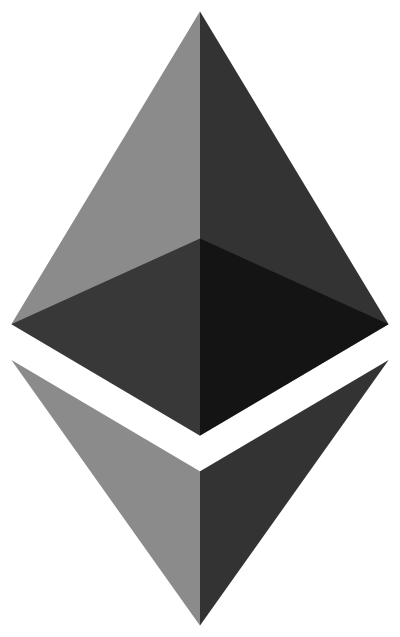
\includegraphics[height=0.2\textheight]{400px-Ethereum_logo.svg} \begin{Huge}
                                                                             Ethereum
        \end{Huge}

        \begin{itemize}
            \item Beginn: 2015,
            \item Entwickler: Vitalik Buterin, Gavin Wood, Jeffrey Wilcke
            \item Coin: Ether, Symbol: ETH
            \item Web: \href{https://ethereum.org/}{ethereum.org}
            \item Zweitgrösste Kryptowährung (nach Bitcoin)
        \end{itemize}
    \end{frame}


    \begin{frame}{Ethereum}{Coins}
        \begin{itemize}
            \item Anzahl Coins im Umlauf 120 Mio (Stand: Februar 2022)
            \item Maximale Anzahl: Unbeschränkt, In Zukunft jedoch deflationär
            \item Momentaner ETH-Preis: 3000 USD
        \end{itemize}
    \end{frame}


    \begin{frame}{Ethereum}{Blockchain}
        \begin{itemize}
            \item Consensus: Proof-of-Work
            \item Blockchain-Grösse 800 GB (Stand: 2021)
            \item Mining: Ethash
            \item \emph{Problem}: Transaktionen sind teuer (Gas Price) und langsam (Minuten)
        \end{itemize}
    \end{frame}

    \begin{frame}{Ethereum}{Blockchain}
        \begin{itemize}
            \item DApps (Decentralized Apps)
            \item Smart Contracts, Prog. Sprache: \emph{Solidity}
            \item Ethereum Virtual Machine (EVM)
            \item Eco-System
            \begin{itemize}
                \item EIP: Ethereum Improvement Proposals
                \item ECR: Ethereum Request for Comments
            \end{itemize}
        \end{itemize}
    \end{frame}

    \begin{frame}{Ethereum}{Roadmap}
        \begin{itemize}
            \item Neuer Consensus 2022: Proof-of-Stake
            \item Layer 2: Schnellere und günstigere Transaktionen
            \item Rollups: Transaktionen ausserhalb, Resultat wird auf der Blockchain gespeichert
            \item Sidechains: Unabhängige Ethereum Blockchain mit Verbindung zur Haupt-Chain
        \end{itemize}
    \end{frame}


    \begin{frame}
        \frametitle{Ethereum \& Alt-Coins}


        \begin{description}
            \item[Definition] Alt-Coins $=$ \textbf{ERC 20} Contracts $=$ Tokens
            \item[Mehr als 400'000] Tokens sind auf Ethereum deployed.
            \item[Stable Coins] sind Tokens mit realen Werten wie USD, Gold
            \item[Shit Coins] oder auch MIME-Coin eigentlich wertlos
            \item[\href{https://etherscan.io/tokens}{Token Tracker}]
        \end{description}
    \end{frame}


    \begin{frame}
        \frametitle{Alt-Coins Beispiels}


        \begin{description}
            \item[USDT Tether] US Dollar als Token, unbeschränkt, USD hinterlegt.
            \item[PAXG Pax Gold] Coin mit hinterlegten Gold Werten
            \item[NEXO] Zinstoken von der Nexo Bank
            \item[AXS Axie] Currency for games, rewards, staking, NFTs
            \item[SHIB Shiba Inu] Mime Coin, eventuell mit Zukunft.
        \end{description}
    \end{frame}


\end{document}

